\documentclass{article}

\usepackage{geometry}
\geometry{margin=2cm}
\usepackage{graphicx}
\usepackage{hyperref}
\usepackage{amsfonts}

\hypersetup{colorlinks=true, linkcolor=blue, urlcolor=blue}
\urlstyle{same}
\begin{document}
	
	\author{Aayush Arya}
	\date{(Submitted: \today)}
	\title{}
	
	\maketitle
	
	\hrule
	\begin{center}
		PHY366 Lab Report\\
		Practical: 2 \quad Registration No.: 11912610 \quad Section: G2903
	\end{center}
	\hrule
	
	\section*{Aim}
	To design a non-inverting amplifier circuit an Op-Amp.
	
	\section*{Methods}
	
	We simulate an operational amplifier circuit on the \textsc{MultiSim} platform\footnote{Circuit available publicly at \url{https://www.multisim.com/content/7ZP2r5NA3vzK7DU9bVdrfT/phy366-op-amp-non-inverting/open/}}. It was configured to operate in a non-inverting fashion (see Figure \ref{fig:circuit}).
	\begin{figure}[h!]
		\centering
		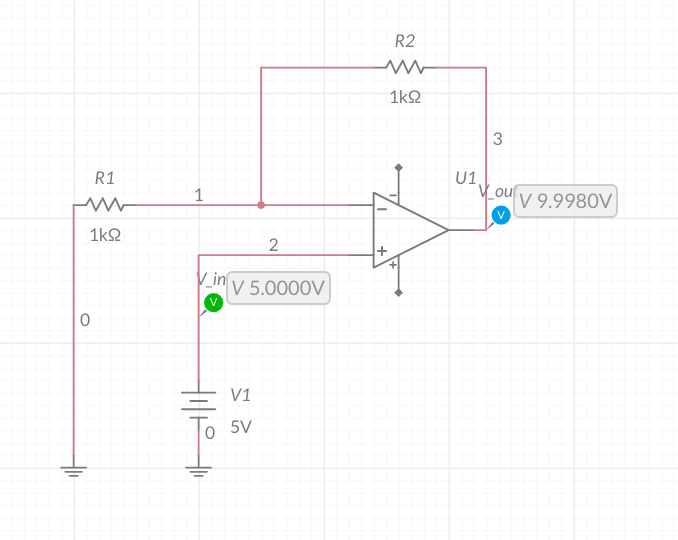
\includegraphics[width=0.6\textwidth]{noninv_circuit}
		\caption{circuit diagram}
		\label{fig:circuit}
	\end{figure}
	
	Theeoretically, the output voltage of an Op-Amp is $$ V_{out} = A_{cl}V_{in}$$
	
	where, for our configuration, the closed loop gain $A_{cl}$ is $$ A_{cl} = 1 + \frac{R_2}{R_1}$$
	
	We check the validity of this result by varying the resistance $R_2$.
	
	\section*{Results and Discussion}
	
	For resistances at input ($R_1 = 1$ $k\Omega$) and output ($R_2 = 1$ $k\Omega$) kept constant, we report the different output DC voltages obtained in Table \ref{tab:obs} obtained by varying the input voltage.
		
		\begin{table}[h!]
			\centering
			\begin{tabular}{|c|c|}
				\hline
				$V_{in}$ (V) & $V_{out}$ (V)\\
				\hline
				
				0.1 & 0.198 \\
				0.5 & 0.998 \\
				2.0 & 3.998 \\
				4.0 & 7.998 \\
				10.0 & 19.998 \\
				25.0 & 50.000 \\
				
				\hline
			\end{tabular}
		\caption{Variation of output potential $V_{out}$ as $R_2$ is varied. }
		\label{tab:obs}
		\end{table}
	
	Note that the output is short of the theoretical expectations due to minor losses. A plot between input and output voltage is shown in Figure \ref{fig:result}.
	
	\begin{figure}[h!]
		\centering
		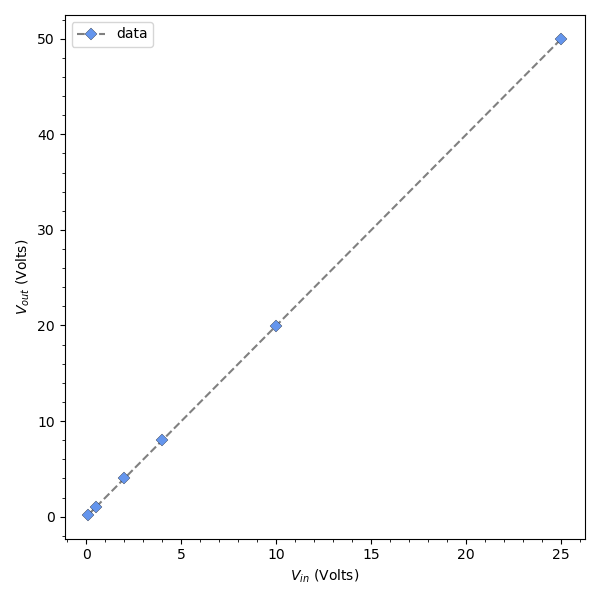
\includegraphics[width=0.5\textwidth]{figure}
		\caption{$V_{out}$ plotted against input voltage $V_{in}$ for constant $R_2/R_1 = 1$, corresponding to $A_{cl} = 2$.}
		\label{fig:result}
	\end{figure}

	The result is therefore, consistent with the straight-line $V_{out}$ expected from the theoretical relation.
\end{document}